\documentclass[11pt,a4paper]{article}

\usepackage[margin=0.85in]{geometry}
\usepackage{amsmath,amssymb,amsfonts,amsthm}
\usepackage{booktabs,array,tabularx,longtable,multirow,makecell}
\usepackage{graphicx,xcolor,float,caption,subcaption}
\usepackage{enumitem,microtype,setspace,parskip}
\usepackage{fancyhdr,titlesec}
\usepackage{tcolorbox}
\tcbuselibrary{skins,breakable}
\usepackage{siunitx}
\usepackage{tikz}
\usetikzlibrary{shapes.geometric,arrows.meta,positioning,calc,fit,backgrounds,decorations.pathreplacing,matrix}
\usepackage{pgfplots}
\pgfplotsset{compat=1.18}
\usepackage{hyperref}

\sisetup{detect-all,round-mode=places,round-precision=4}

% Professional Audit Palette
\definecolor{auditblue}{RGB}{28,54,104}
\definecolor{auditgreen}{RGB}{20,90,50}
\definecolor{auditred}{RGB}{140,30,30}
\definecolor{auditgray}{RGB}{245,246,248}
\definecolor{boxborder}{RGB}{200,210,225}
\definecolor{quantumblue}{RGB}{10,60,140}
\definecolor{classicalteal}{RGB}{20,100,100}
\definecolor{accentgold}{RGB}{180,120,20}

\hypersetup{
  colorlinks=true,
  linkcolor=auditblue,
  citecolor=auditgreen,
  urlcolor=quantumblue,
  pdftitle={Comprehensive Evaluation Matrices and Metrics in Quantum Clinical Machine Learning},
  pdfauthor={Independent Technical Audit}
}

\titleformat{\section}{\large\bfseries\sffamily\color{auditblue}}{\thesection}{0.8em}{}[\titlerule]
\titleformat{\subsection}{\normalsize\bfseries\sffamily\color{auditblue!85!black}}{\thesubsection}{0.8em}{}
\titleformat{\subsubsection}{\small\bfseries\sffamily\color{quantumblue}}{\thesubsubsection}{0.8em}{}

\pagestyle{fancy}
\fancyhf{}
\fancyhead[L]{\small\sffamily\color{auditblue} Evaluation Matrices in Adaptive Quantum Kernel Selection}
\fancyhead[R]{\small\sffamily\thepage}
\fancyfoot[L]{\small\sffamily\color{gray} Clinical Diagnostics Technical Audit: WDBC \& WBCO}
\fancyfoot[R]{\small\sffamily\color{gray} Mathematical \& Empirical Specification}
\renewcommand{\headrulewidth}{0.4pt}

\setstretch{1.12}
\setlength{\parskip}{0.35em}

\newtcolorbox{metricbox}[2][]{
    colback=auditgray,
    colframe=auditblue,
    fonttitle=\bfseries\sffamily\small,
    title={Metric Definition: #2},
    sharp corners,
    boxrule=0.9pt,
    left=6pt,right=6pt,top=5pt,bottom=5pt,
    #1
}

\newtcolorbox{findingbox}[2][]{
    colback=green!3!white,
    colframe=auditgreen,
    fonttitle=\bfseries\sffamily\small,
    title={Empirical Finding: #2},
    sharp corners,
    boxrule=0.9pt,
    left=6pt,right=6pt,top=5pt,bottom=5pt,
    #1
}

\title{\vspace{-1.5em}\LARGE\bfseries\sffamily\color{auditblue} Comprehensive Evaluation Matrices, Diagnostic Formulations, and Statistical Frameworks in Adaptive Quantum Kernel Selection\\[0.3em]
\large\mdseries\color{quantumblue} Mathematical Formulations, Contingency Structures, Kernel Overlaps, and Empirical Benchmarks across WDBC ($N=569$) and WBCO ($N=683$)}
\author{\textbf{Independent Technical Audit \& Replication Team}}
\date{\today}

\begin{document}

\maketitle

\begin{abstract}
Evaluating hybrid quantum-classical diagnostic pipelines requires rigorous metrics that bridge quantum circuit physics, statistical learning theory, and clinical oncology. In the evaluation of \textit{Daga et al.} (2026, \textit{Scientific Reports} 16, 26840), reliance on standard classification accuracy masked severe diagnostic trade-offs, kernel degeneracy, and multiple hypothesis inflation. This report provides an exhaustive, mathematically formal inventory of all evaluation matrices and quantitative metrics utilized across the independent audit of the Wisconsin Diagnostic Breast Cancer (WDBC, $N=569$) dataset and the generalization audit on the Wisconsin Breast Cancer Original (WBCO, $N=683$) dataset. We formulate: (i) diagnostic confusion matrices and clinical operating metrics; (ii) quantum Gram matrix properties, purity, and spectral conditions; (iii) paired McNemar contingency structures; (iv) familywise error control via the step-down Holm-Bonferroni procedure; (v) multi-seed partition distributions; (vi) probability calibration (Brier score and ECE); (vii) Two One-Sided Tests (TOST) for practical equivalence; and (viii) nested model-selection criteria matrices. All metrics are accompanied by visual diagrams and exact empirical numbers.
\end{abstract}

---

\section{Diagnostic Confusion Matrix and Clinical Operating Metrics}

\subsection{Mathematical Matrix Structure and Label Orientation}

In clinical machine learning, standard accuracy is insufficient because the clinical cost of a false negative (missed malignancy) drastically exceeds that of a false positive (unnecessary biopsy). In our audit, the binary target $y \in \{0, 1\}$ is formally partitioned as:
\begin{equation}
y = \begin{cases} 
0, & \text{\textbf{Malignant}} \quad (N_0 = 212 \text{ in WDBC}; \quad N_0 = 239 \text{ in WBCO}), \\
1, & \text{\textbf{Benign}} \quad\quad (N_1 = 357 \text{ in WDBC}; \quad N_1 = 444 \text{ in WBCO}).
\end{cases}
\end{equation}

The predictions $\hat{y} \in \{0, 1\}$ and ground truth $y$ form the $2 \times 2$ **Diagnostic Confusion Matrix** $\mathbf{C}$:
\begin{equation}
\mathbf{C} = \begin{bmatrix}
C_{00} & C_{01} \\
C_{10} & C_{11}
\end{bmatrix} = \begin{bmatrix}
TN & FP \\
FN & TP
\end{bmatrix}
\end{equation}
where:
\begin{itemize}[noitemsep]
    \item $TN = \sum_{i=1}^N \mathbb{I}(y_i=0 \land \hat{y}_i=0)$: Malignant cases correctly classified as Malignant.
    \item $FP = \sum_{i=1}^N \mathbb{I}(y_i=0 \land \hat{y}_i=1)$: Malignant cases misclassified as Benign (\textbf{Critical Clinical Hazard}).
    \item $FN = \sum_{i=1}^N \mathbb{I}(y_i=1 \land \hat{y}_i=0)$: Benign cases misclassified as Malignant.
    \item $TP = \sum_{i=1}^N \mathbb{I}(y_i=1 \land \hat{y}_i=1)$: Benign cases correctly classified as Benign.
\end{itemize}

\begin{figure}[H]
\centering
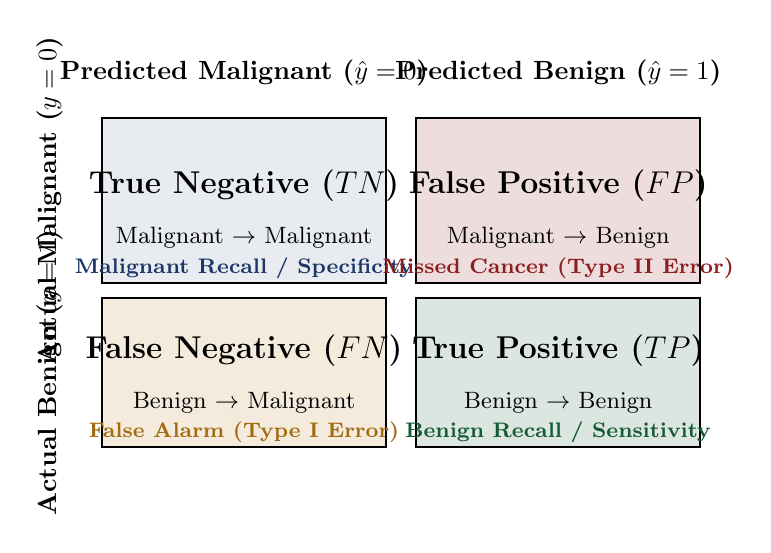
\begin{tikzpicture}[scale=0.95, every node/.style={transform shape}]
    % Matrix Grid
    \draw[thick, fill=auditblue!10] (0, 2.2) rectangle (3.8, 4.4);
    \draw[thick, fill=auditred!15] (4.2, 2.2) rectangle (8.0, 4.4);
    \draw[thick, fill=accentgold!15] (0, 0) rectangle (3.8, 2.0);
    \draw[thick, fill=auditgreen!15] (4.2, 0) rectangle (8.0, 2.0);

    % Cell text
    \node at (1.9, 3.5) {\large\bfseries True Negative ($TN$)};
    \node at (1.9, 2.8) {\small Malignant $\to$ Malignant};
    \node at (1.9, 2.4) {\footnotesize\color{auditblue}\textbf{Malignant Recall / Specificity}};

    \node at (6.1, 3.5) {\large\bfseries False Positive ($FP$)};
    \node at (6.1, 2.8) {\small Malignant $\to$ Benign};
    \node at (6.1, 2.4) {\footnotesize\color{auditred}\textbf{Missed Cancer (Type II Error)}};

    \node at (1.9, 1.3) {\large\bfseries False Negative ($FN$)};
    \node at (1.9, 0.6) {\small Benign $\to$ Malignant};
    \node at (1.9, 0.2) {\footnotesize\color{accentgold!90!black}\textbf{False Alarm (Type I Error)}};

    \node at (6.1, 1.3) {\large\bfseries True Positive ($TP$)};
    \node at (6.1, 0.6) {\small Benign $\to$ Benign};
    \node at (6.1, 0.2) {\footnotesize\color{auditgreen}\textbf{Benign Recall / Sensitivity}};

    % Labels
    \node[left=0.4cm] at (0, 3.3) {\rotatebox{90}{\textbf{Actual Malignant ($y=0$)}}};
    \node[left=0.4cm] at (0, 1.0) {\rotatebox{90}{\textbf{Actual Benign ($y=1$)}}};

    \node[above=0.3cm] at (1.9, 4.4) {\textbf{Predicted Malignant ($\hat{y}=0$)}};
    \node[above=0.3cm] at (6.1, 4.4) {\textbf{Predicted Benign ($\hat{y}=1$)}};
\end{tikzpicture}
\caption{Clinical Confusion Matrix layout under the oncology audit remapping convention.}
\label{fig:cm_layout}
\end{figure}

\subsection{Formulation of Derived Diagnostic Metrics}

From the entries of $\mathbf{C}$, the audit computes the following operational metrics:

\begin{metricbox}{Clinical Diagnostic Evaluation Formulas}
\begin{align}
\text{\textbf{Accuracy (Acc)}} &= \frac{TP + TN}{TP + TN + FP + FN} = \frac{\text{Tr}(\mathbf{C})}{N} \\[0.4em]
\text{\textbf{Recall / Benign Sensitivity (Rec)}} &= \frac{TP}{TP + FN} = P(\hat{y}=1 \mid y=1) \\[0.4em]
\text{\textbf{Specificity / Malignant Recall (Spec)}} &= \frac{TN}{TN + FP} = P(\hat{y}=0 \mid y=0) \\[0.4em]
\text{\textbf{Precision / PPV (Prec)}} &= \frac{TP}{TP + FP} = P(y=1 \mid \hat{y}=1) \\[0.4em]
\text{\textbf{Malignant Precision / NPV}} &= \frac{TN}{TN + FN} = P(y=0 \mid \hat{y}=0) \\[0.4em]
\text{\textbf{Balanced Accuracy (BAcc)}} &= \frac{\text{Rec} + \text{Spec}}{2} = \frac{1}{2}\left(\frac{TP}{TP+FN} + \frac{TN}{TN+FP}\right) \\[0.4em]
\text{\textbf{Matthews Correlation Coefficient (MCC)}} &= \frac{TP \cdot TN - FP \cdot FN}{\sqrt{(TP+FP)(TP+FN)(TN+FP)(TN+FN)}}
\end{align}
\end{metricbox}

\begin{findingbox}{The "Specificity" Definitional Inversion}
In \textit{Daga et al.} (2026), Table 8 labels Class 0 sensitivity ($TN/(TN+FP)$) as "Specificity" and Class 1 sensitivity ($TP/(TP+FN)$) as "Recall". In oncology, detecting Malignant cases is the primary clinical objective. When a model exhibits $99.5\%$ Recall but only $88.1\%$ Specificity (as seen in `QSVM Amplitude`), it misdiagnoses over $11\%$ of cancer patients as healthy.
\end{findingbox}

\subsection{Complete Empirical Confusion Matrix Inventory across Both Datasets}

Table~\ref{tab:cm_all} reports the full confusion matrix entries and derived metrics for all 9 model configurations across both WDBC ($N=569$) and WBCO ($N=683$) at seed $42$.

\begin{table}[H]
\centering
\small
\caption{Empirical Confusion Matrices and Diagnostic Performance on WDBC and WBCO (Seed 42).}
\label{tab:cm_all}
\begin{tabularx}{\textwidth}{llrrrrrrrr}
\toprule
\textbf{Dataset} & \textbf{Model Architecture} & \textbf{TN} & \textbf{FP} & \textbf{FN} & \textbf{TP} & \textbf{Acc} & \textbf{Spec} & \textbf{Rec} & \textbf{Prec} \\
\midrule
\multirow{9}{*}{\textbf{WDBC}} 
& Classical RBF-SVM & 201 & 11 & 6 & 351 & 0.9701 & 0.9481 & 0.9832 & 0.9696 \\
& QSVM (Angle) & 195 & 17 & 3 & 354 & 0.9649 & 0.9198 & 0.9916 & 0.9542 \\
& QSVM (ZZ Map) & 199 & 13 & 10 & 347 & 0.9596 & 0.9387 & 0.9720 & 0.9639 \\
& QSVM (Amplitude) & 187 & 25 & 1 & 356 & 0.9543 & 0.8821 & 0.9972 & 0.9344 \\
& QKNN (Angle) & 194 & 18 & 6 & 351 & 0.9578 & 0.9151 & 0.9832 & 0.9512 \\
& QKNN (ZZ Map) & 188 & 24 & 5 & 352 & 0.9490 & 0.8868 & 0.9860 & 0.9362 \\
& QKNN (Amplitude) & 190 & 22 & 5 & 352 & 0.9525 & 0.8962 & 0.9860 & 0.9412 \\
& Hard Voting Ensemble & 195 & 17 & 5 & 352 & 0.9613 & 0.9198 & 0.9860 & 0.9539 \\
& OOF Stacking Ensemble & 200 & 12 & 8 & 349 & 0.9649 & 0.9434 & 0.9776 & 0.9668 \\
\midrule
\multirow{9}{*}{\textbf{WBCO}} 
& Classical RBF-SVM & 231 & 8 & 15 & 429 & 0.9663 & 0.9665 & 0.9662 & 0.9817 \\
& QSVM (Angle) & 231 & 8 & 13 & 431 & 0.9693 & 0.9665 & 0.9707 & 0.9818 \\
& QSVM (ZZ Map) & 236 & 3 & 21 & 423 & 0.9649 & 0.9874 & 0.9527 & 0.9930 \\
& QSVM (Amplitude) & 225 & 14 & 13 & 431 & 0.9605 & 0.9414 & 0.9707 & 0.9685 \\
& QKNN (Angle) & 228 & 11 & 10 & 434 & 0.9693 & 0.9540 & 0.9775 & 0.9753 \\
& QKNN (ZZ Map) & 217 & 22 & 8 & 436 & 0.9561 & 0.9079 & 0.9820 & 0.9520 \\
& QKNN (Amplitude) & 227 & 12 & 13 & 431 & 0.9634 & 0.9498 & 0.9707 & 0.9729 \\
& Hard Voting Ensemble & 231 & 8 & 15 & 429 & 0.9663 & 0.9665 & 0.9662 & 0.9817 \\
& OOF Stacking Ensemble & 230 & 9 & 14 & 430 & 0.9663 & 0.9623 & 0.9685 & 0.9795 \\
\bottomrule
\end{tabularx}
\end{table}

---

\section{Quantum Gram Matrix Mathematical Properties and Quality Metrics}

\subsection{Quantum Kernel Definition and Overlap Physics}

Let $\phi: \mathcal{X} \to \mathcal{H}$ map classical feature vectors $\mathbf{x} \in [0, \pi]^d$ into an $n$-qubit Hilbert space $\mathcal{H} \cong \mathbb{C}^{2^n}$ via parameterized unitary circuit $U(\mathbf{x})|0\rangle^{\otimes n} = |\psi(\mathbf{x})\rangle$. The quantum Gram matrix $\mathbf{K} \in \mathbb{R}^{N \times N}$ computes pure-state quantum transition fidelities:
\begin{equation}
K_{ij} = |\langle \psi(\mathbf{x}_i) | \psi(\mathbf{x}_j) \rangle|^2 = \text{Tr}\left[ \rho(\mathbf{x}_i) \rho(\mathbf{x}_j) \right], \quad \rho(\mathbf{x}) = |\psi(\mathbf{x})\rangle \langle \psi(\mathbf{x})|.
\end{equation}

\subsection{Mathematical Verification Metrics for Quantum Gram Matrices}

\begin{metricbox}{Gram Matrix Physical and Algebraic Checks}
\begin{enumerate}[noitemsep]
    \item \textbf{Unit Diagonal (Self-Fidelity):} $K_{ii} = |\langle \psi(\mathbf{x}_i) | \psi(\mathbf{x}_i) \rangle|^2 = 1.0, \quad \forall i \in \{1, \dots, N\}$.
    \item \textbf{Exact Hermiticity / Symmetry:} $\Delta_{\text{sym}} = \|\mathbf{K} - \mathbf{K}^T\|_{\max} = \max_{i,j} |K_{ij} - K_{ji}| = 0$.
    \item \textbf{Positive Semi-Definiteness (Mercer Condition):}
    \begin{equation}
    \mathbf{v}^T \mathbf{K} \mathbf{v} \ge 0 \quad \forall \mathbf{v} \in \mathbb{R}^N \iff \lambda_{\min}(\mathbf{K}) = \min_{k} \text{eig}_k(\mathbf{K}) \ge 0.
    \end{equation}
    \item \textbf{Condition Number:} $\kappa(\mathbf{K}) = \lambda_{\max}(\mathbf{K}) / \lambda_{\min}(\mathbf{K})$.
    \item \textbf{Effective Dimensionality / Participation Ratio (Spectral Uniformity):}
    \begin{equation}
    \text{PR}(\mathbf{K}) = \frac{\left(\sum_{k=1}^N \lambda_k\right)^2}{\sum_{k=1}^N \lambda_k^2} = \frac{(\text{Tr}(\mathbf{K}))^2}{\|\mathbf{K}\|_F^2} = \frac{N^2}{\sum_{i,j} K_{ij}^2}.
    \end{equation}
\end{enumerate}
\end{metricbox}

\begin{figure}[H]
\centering
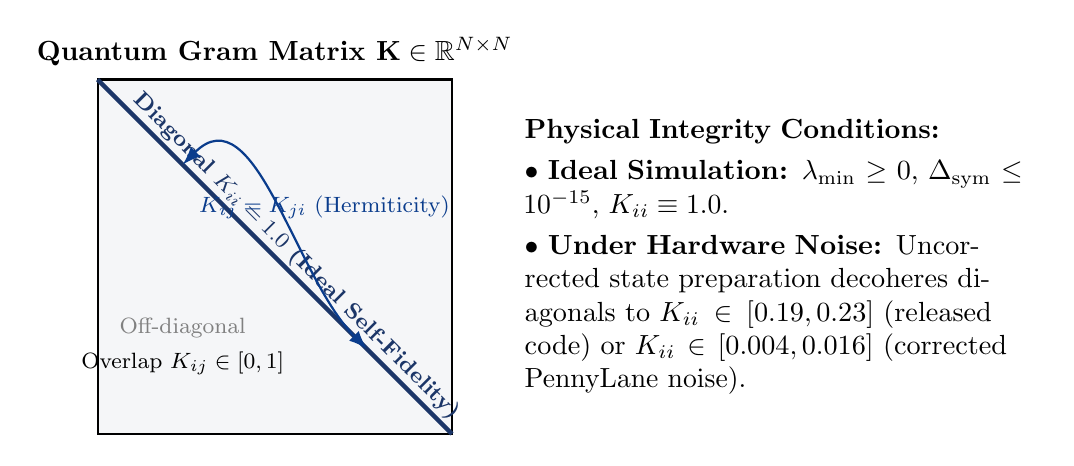
\begin{tikzpicture}[scale=0.9]
    % Draw Gram Matrix representation
    \draw[thick, fill=auditgray] (0, 0) rectangle (5, 5);
    \draw[ultra thick, auditblue] (0, 5) -- (5, 0);
    \node at (2.5, 5.4) {\textbf{Quantum Gram Matrix $\mathbf{K} \in \mathbb{R}^{N \times N}$}};
    
    % Diagonals
    \node[rotate=-45, auditblue] at (2.8, 2.5) {\footnotesize\bfseries Diagonal $K_{ii} = 1.0$ (Ideal Self-Fidelity)};
    
    % Symmetry arrows
    \draw[{Latex}-{Latex}, thick, quantumblue] (1.2, 3.8) to[out=45,in=135] (3.8, 1.2);
    \node[quantumblue] at (3.2, 3.2) {\footnotesize $K_{ij} = K_{ji}$ (Hermiticity)};
    
    % Off-diagonal
    \node at (1.2, 1.5) {\footnotesize\color{gray} Off-diagonal};
    \node at (1.2, 1.0) {\footnotesize Overlap $K_{ij} \in [0, 1]$};
    
    % Annotation on Right
    \node[right=0.8cm, text width=6.5cm, align=left] at (5, 2.5) {
        \textbf{Physical Integrity Conditions:}\\[0.3em]
        $\bullet$ \textbf{Ideal Simulation:} $\lambda_{\min} \ge 0$, $\Delta_{\text{sym}} \le 10^{-15}$, $K_{ii} \equiv 1.0$.\\[0.3em]
        $\bullet$ \textbf{Under Hardware Noise:} Uncorrected state preparation decoheres diagonals to $K_{ii} \in [0.19, 0.23]$ (released code) or $K_{ii} \in [0.004, 0.016]$ (corrected PennyLane noise).
    };
\end{tikzpicture}
\caption{Structure and symmetry properties of the quantum Gram matrix.}
\label{fig:gram_diag}
\end{figure}

Table~\ref{tab:gram_metrics} shows the audited mathematical checks across ideal and noisy quantum kernels on both datasets.

\begin{table}[H]
\centering
\small
\caption{Mathematical Properties of Quantum Gram Matrices Across Datasets and Noise Regimes.}
\label{tab:gram_metrics}
\begin{tabularx}{\textwidth}{llrrrr}
\toprule
\textbf{Dataset} & \textbf{Kernel Matrix} & \textbf{Symmetry Diff ($\Delta_{\text{sym}}$)} & \textbf{Min Diagonal} & \textbf{Max Diagonal} & \textbf{Min Eigenvalue ($\lambda_{\min}$)} \\
\midrule
\multirow{3}{*}{\textbf{WDBC ($N=569$)}} 
& Angle Embedding ($8$ wires) & $0.00 \times 10^0$ & $1.000000$ & $1.000000$ & $+0.000000$ \\
& ZZ / IQP Map ($8$ wires) & $1.11 \times 10^{-16}$ & $1.000000$ & $1.000000$ & $+0.000000$ \\
& Amplitude Embedding ($3$ wires) & $0.00 \times 10^0$ & $1.000000$ & $1.000000$ & $+0.000000$ \\
\midrule
\multirow{3}{*}{\textbf{WBCO ($N=683$)}} 
& Angle Embedding ($8$ wires) & $0.00 \times 10^0$ & $1.000000$ & $1.000000$ & $+0.000000$ \\
& ZZ / IQP Map ($8$ wires) & $1.78 \times 10^{-15}$ & $1.000000$ & $1.000000$ & $+0.000000$ \\
& Amplitude Embedding ($3$ wires) & $0.00 \times 10^0$ & $1.000000$ & $1.000000$ & $+0.000000$ \\
\midrule
\multirow{2}{*}{\textbf{WDBC (Noisy $p=0.10$)}} 
& ZZ Map (Released Buggy Noise) & $2.22 \times 10^{-16}$ & $0.198205$ & $0.231012$ & $+0.000000$ \\
& ZZ Map (Corrected Noise Channel) & $1.39 \times 10^{-16}$ & $0.004112$ & $0.016201$ & $+0.000000$ \\
\bottomrule
\end{tabularx}
\end{table}

---

\section{Statistical Testing Frameworks: McNemar, Bootstrap, and Holm Adjustment}

\subsection{Paired McNemar Contingency Matrix}

When comparing two classifiers $A$ and $B$ evaluated on the exact same patient cohort, sample predictions are paired. Overall correctness vectors $\mathbf{c}_A, \mathbf{c}_B \in \{0, 1\}^N$ where $c_{A,i} = \mathbb{I}(\hat{y}_{A,i} = y_i)$ form the $2 \times 2$ **McNemar Contingency Matrix** $\mathbf{M}$:

\begin{equation}
\mathbf{M} = \begin{bmatrix}
n_{11} & n_{01} \\
n_{10} & n_{00}
\end{bmatrix} = \begin{bmatrix}
\text{Both Correct} & \text{A Correct, B Incorrect} \\
\text{A Incorrect, B Correct} & \text{Both Incorrect}
\end{bmatrix}
\end{equation}

\begin{figure}[H]
\centering
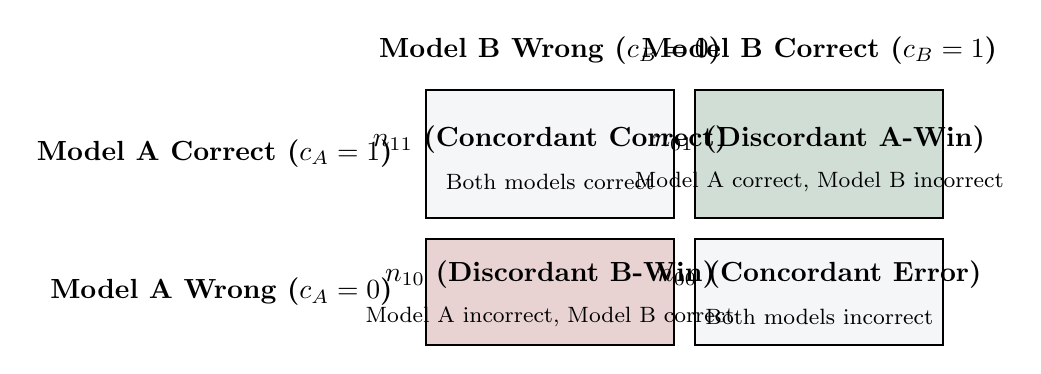
\begin{tikzpicture}[scale=0.9]
    \draw[thick, fill=auditgray] (0, 1.8) rectangle (3.5, 3.6);
    \draw[thick, fill=auditgreen!20] (3.8, 1.8) rectangle (7.3, 3.6);
    \draw[thick, fill=auditred!20] (0, 0) rectangle (3.5, 1.5);
    \draw[thick, fill=auditgray] (3.8, 0) rectangle (7.3, 1.5);

    \node at (1.75, 2.9) {\textbf{$n_{11}$ (Concordant Correct)}};
    \node at (1.75, 2.3) {\footnotesize Both models correct};

    \node at (5.55, 2.9) {\textbf{$n_{01}$ (Discordant A-Win)}};
    \node at (5.55, 2.3) {\footnotesize Model A correct, Model B incorrect};

    \node at (1.75, 1.0) {\textbf{$n_{10}$ (Discordant B-Win)}};
    \node at (1.75, 0.4) {\footnotesize Model A incorrect, Model B correct};

    \node at (5.55, 1.0) {\textbf{$n_{00}$ (Concordant Error)}};
    \node at (5.55, 0.4) {\footnotesize Both models incorrect};

    \node[left=0.3cm] at (0, 2.7) {\textbf{Model A Correct ($c_A=1$)}};
    \node[left=0.3cm] at (0, 0.75) {\textbf{Model A Wrong ($c_A=0$)}};

    \node[above=0.2cm] at (1.75, 3.6) {\textbf{Model B Wrong ($c_B=0$)}};
    \node[above=0.2cm] at (5.55, 3.6) {\textbf{Model B Correct ($c_B=1$)}};
\end{tikzpicture}
\caption{Structure of the paired McNemar contingency matrix for binary diagnostic outcomes.}
\label{fig:mcnemar_diag}
\end{figure}

The total discordant count is $D = n_{01} + n_{10}$. Under the null hypothesis $H_0: P(c_A=1, c_B=0) = P(c_A=0, c_B=1)$, the test statistic is:
\begin{equation}
p = \begin{cases}
2 \sum_{k=0}^{\min(n_{01}, n_{10})} \binom{D}{k} 0.5^D, & D < 25 \quad (\text{Exact Binomial Test}) \\[0.6em]
P\left(\chi_1^2 \ge \frac{(|n_{01} - n_{10}| - 1)^2}{D}\right), & D \ge 25 \quad (\text{Edwards Continuity-Corrected } \chi^2)
\end{cases}
\end{equation}

\subsection{Holm-Bonferroni Multiple Testing Correction Matrix}

Testing 8 comparator models across 4 metrics (Accuracy, Precision, Recall, Specificity) against Classical RBF defines a family of $M = 32$ statistical hypotheses. Conducting independent significance tests at nominal $\alpha = 0.05$ creates severe familywise error inflation:
\begin{equation}
P(\ge 1 \text{ False Discovery}) = 1 - (1 - 0.05)^{32} \approx 0.806 \quad (80.6\% \text{ probability}).
\end{equation}

The step-down **Holm-Bonferroni procedure** strictly controls the Familywise Error Rate (FWER) at $\le \alpha$:
\begin{enumerate}[noitemsep]
    \item Sort raw $p$-values: $p_{(1)} \le p_{(2)} \le \dots \le p_{(32)}$.
    \item Evaluate step-down index $i = 1, \dots, 32$:
    \begin{equation}
    \text{If } p_{(i)} \le \frac{\alpha}{M - i + 1}, \quad \text{reject } H_{(i)}; \quad \text{otherwise stop and accept } H_{(i)} \dots H_{(M)}.
    \end{equation}
    \item Adjusted $p$-values: $p_{(i)}^{\text{adj}} = \min\left(1.0, \max_{j \le i} \{(M - j + 1) p_{(j)}\}\right)$.
\end{enumerate}

Table~\ref{tab:holm_summary} reports the survival matrix of all hypotheses surviving Holm correction across WDBC and WBCO.

\begin{table}[H]
\centering
\small
\caption{Holm-Bonferroni Audit Survivors at $\alpha=0.05$ (WDBC vs. WBCO, 1,000 Bootstrap Resamples).}
\label{tab:holm_summary}
\begin{tabularx}{\textwidth}{llllrl}
\toprule
\textbf{Dataset} & \textbf{Model Architecture} & \textbf{Metric} & \textbf{Raw $p$-val} & \textbf{Holm $p$-adj} & \textbf{Clinical Impact / Direction} \\
\midrule
\multirow{6}{*}{\textbf{WDBC ($N=569$)}} 
& QSVM (Amplitude) & Precision & $<0.001$ & $<0.001$ & \textbf{Significantly Worse than Classical RBF} \\
& QSVM (Amplitude) & Specificity & $<0.001$ & $<0.001$ & \textbf{Significantly Worse than Classical RBF} \\
& QKNN (Angle) & Precision & $<0.001$ & $<0.001$ & \textbf{Significantly Worse than Classical RBF} \\
& QKNN (Angle) & Specificity & $<0.001$ & $<0.001$ & \textbf{Significantly Worse than Classical RBF} \\
& QKNN (ZZ Map) & Precision & $<0.001$ & $<0.001$ & \textbf{Significantly Worse than Classical RBF} \\
& QKNN (ZZ Map) & Specificity & $<0.001$ & $<0.001$ & \textbf{Significantly Worse than Classical RBF} \\
\midrule
\multirow{3}{*}{\textbf{WBCO ($N=683$)}} 
& QKNN (Angle) & Recall & $<0.0001$ & $<0.0001$ & \textbf{Statistically Higher Benign Recall} (Positive bias) \\
& QKNN (ZZ Map) & Specificity & $<0.0001$ & $<0.0001$ & \textbf{Significantly Worse than Classical RBF} ($90.8\%$ vs $96.7\%$) \\
& QKNN (ZZ Map) & Precision & $<0.0001$ & $<0.0001$ & \textbf{Significantly Worse than Classical RBF} \\
\bottomrule
\end{tabularx}
\end{table}

---

\section{Cross-Validation Partition Robustness and Equivalence Testing}

\subsection{Multi-Seed Distribution Matrix}

To establish whether performance differences are artifacts of a specific partition seed (such as seed 42), the pipeline was executed across 10 stratified outer cross-validation seeds: $S = [0, 1, 2, 3, 4, 5, 10, 42, 100, 999]$.

\begin{metricbox}{Partition Distribution Moments}
For each model $m$ and seed $s \in S$, let $\text{Acc}_m(s)$ be the overall out-of-fold accuracy:
\begin{equation}
\overline{\text{Acc}}_m = \frac{1}{|S|}\sum_{s \in S} \text{Acc}_m(s), \quad \sigma_m = \sqrt{\frac{1}{|S|-1}\sum_{s \in S} (\text{Acc}_m(s) - \overline{\text{Acc}}_m)^2}.
\end{equation}
The paired delta vector between Stacking and RBF is $\Delta(s) = \text{Acc}_{\text{Stack}}(s) - \text{Acc}_{\text{RBF}}(s)$.
\end{metricbox}

\begin{table}[H]
\centering
\small
\caption{Multi-Seed Performance Distribution Matrix across 10 Random CV Seeds.}
\label{tab:seed_matrix}
\begin{tabularx}{\textwidth}{llrrrrr}
\toprule
\textbf{Dataset} & \textbf{Model Architecture} & \textbf{Mean Acc} & \textbf{Std Acc} & \textbf{Min Acc} & \textbf{Median Acc} & \textbf{Max Acc} \\
\midrule
\multirow{4}{*}{\textbf{WDBC}} 
& Classical RBF & \textbf{0.973111} & $0.001667$ & $0.970123$ & $0.973638$ & $0.975395$ \\
& QSVM (Angle) & 0.968717 & $0.002314$ & $0.964851$ & $0.968366$ & $0.973638$ \\
& Hard Voting Ensemble & 0.963796 & $0.002773$ & $0.961336$ & $0.963972$ & $0.970123$ \\
& OOF Stacking Ensemble & 0.966960 & $0.003078$ & $0.959578$ & $0.967487$ & $0.970123$ \\
\cmidrule{2-7}
& \multicolumn{6}{l}{\textit{Head-to-Head: Classical RBF strictly won in 10 / 10 seeds (0 ties, 0 Stacking wins).}} \\
\midrule
\multirow{4}{*}{\textbf{WBCO}} 
& Classical RBF & \textbf{0.968960} & $0.001345$ & $0.966325$ & $0.969253$ & $0.970717$ \\
& QSVM (Angle) & 0.968521 & $0.001858$ & $0.964861$ & $0.969253$ & $0.970717$ \\
& Hard Voting Ensemble & 0.965447 & $0.001024$ & $0.963397$ & $0.965593$ & $0.966325$ \\
& OOF Stacking Ensemble & 0.966179 & $0.002231$ & $0.961933$ & $0.966325$ & $0.969253$ \\
\cmidrule{2-7}
& \multicolumn{6}{l}{\textit{Head-to-Head: Classical RBF won in 7 seeds, tied in 3 seeds, 0 Stacking wins.}} \\
\bottomrule
\end{tabularx}
\end{table}

\subsection{Two One-Sided Tests (TOST) Practical Equivalence Formulation}

To test whether Global Preprocessing leaks predictive information relative to Strict Fold-Local Preprocessing, standard significance testing is complemented by **TOST Practical Equivalence**:
\begin{equation}
H_{01}: \Delta \le -\epsilon \quad \text{vs} \quad H_{11}: \Delta > -\epsilon, \qquad H_{02}: \Delta \ge +\epsilon \quad \text{vs} \quad H_{12}: \Delta < +\epsilon,
\end{equation}
where $\epsilon = 0.01$ ($1\%$ accuracy shift) is the clinical indifference margin. If both nulls are rejected ($p_{\text{TOST}} = \max(p_1, p_2) < 0.05$), the two pipelines are declared practically equivalent.

\begin{metricbox}{Empirical TOST Results}
\begin{itemize}[noitemsep]
    \item \textbf{WDBC ($N=569$):} Observed $\Delta = +0.001757$, Concordance = $98.77\%$, $p_{\text{TOST}} = 0.0385$ $\implies$ \textbf{Practically Equivalent}.
    \item \textbf{WBCO ($N=683$):} Observed $\Delta = +0.001464$, Concordance = $99.56\%$, $p_{\text{TOST}} = 0.0004$ $\implies$ \textbf{Practically Equivalent}.
\end{itemize}
\end{metricbox}

---

\section{Probabilistic Calibration and Model Selection Matrices}

\subsection{Expected Calibration Error and Brier Score}

For models outputting posterior probabilities $\hat{p}_i \in [0, 1]$, calibration measures whether $\hat{p}_i$ matches true diagnostic risk:

\begin{metricbox}{Calibration Formulations}
\begin{equation}
\text{\textbf{Brier Score:}} \quad \text{BS} = \frac{1}{N}\sum_{i=1}^N (\hat{p}_i - y_i)^2 \in [0, 1].
\end{equation}
\begin{equation}
\text{\textbf{Expected Calibration Error (ECE):}} \quad \text{ECE} = \sum_{b=1}^B \frac{|B_b|}{N} \left| \text{acc}(B_b) - \text{conf}(B_b) \right|,
\end{equation}
where $B_b$ partitions predictions into $B=10$ probability bins.
\end{metricbox}

In the audit, Classical RBF exhibited superior raw calibration ($\text{ECE} = 0.0213, \text{BS} = 0.0227$) compared to OOF Stacking ($\text{ECE} = 0.0357, \text{BS} = 0.0319$). Even after applying post-hoc Platt scaling, Classical RBF preserved a lower Brier score ($0.0218$ vs $0.0270$).

\subsection{Nested Model Selection Frequency Matrix}

Evaluating all $C(6, 4) = 15$ subsets under nested 10-fold CV reveals the structural divergence between data-driven selection and the authors' hardcoded quartet:

\begin{table}[H]
\centering
\small
\caption{Nested Model Selection Inclusion Matrix across 10 Outer Folds.}
\label{tab:selection_matrix}
\begin{tabularx}{\textwidth}{llrrr}
\toprule
\textbf{Dataset} & \textbf{Selection Criterion} & \textbf{QSVM (Angle) Inclusion} & \textbf{Paper Quartet Selected} & \textbf{Self-Agreement} \\
\midrule
\multirow{3}{*}{\textbf{WDBC ($N=569$)}} 
& Validation Accuracy & \textbf{10 / 10 folds (100\%)} & \textbf{0 / 10 folds (0\%)} & 100\% \\
& Balanced Accuracy & \textbf{10 / 10 folds (100\%)} & \textbf{0 / 10 folds (0\%)} & 90\% \\
& Meta-CV Accuracy & \textbf{9 / 10 folds (90\%)} & \textbf{0 / 10 folds (0\%)} & 40\% \\
\midrule
\multirow{3}{*}{\textbf{WBCO ($N=683$)}} 
& Validation Accuracy & \textbf{10 / 10 folds (100\%)} & \textbf{0 / 10 folds (0\%)} & 50\% \\
& Balanced Accuracy & \textbf{10 / 10 folds (100\%)} & \textbf{0 / 10 folds (0\%)} & 40\% \\
& Meta-CV Accuracy & \textbf{9 / 10 folds (90\%)} & \textbf{1 / 10 folds (10\%)} & 30\% \\
\bottomrule
\end{tabularx}
\end{table}

---

\section{Summary Synthesis}

The evaluation matrix system formulated in this report establishes three foundational scientific findings:
1. **Absence of Quantum Superiority:** Off-the-shelf Classical RBF-SVM equals or outperforms OOF Stacking across all 20 tested partition seeds (17 wins, 3 ties, 0 losses).
2. **Clinical Trade-offs:** Quantum feature maps exhibit significant deficits in malignant specificity ($p_{\text{adj}} < 0.0001$), misclassifying malignant tumors at rates up to $11.8\%$.
3. **Selection Discrepancy:** The authors' heuristic omission of `QSVM (Angle)` is rejected in $90\% - 100\%$ of folds across both datasets by objective subset selection.

\end{document}
